% Bibliography is maintained in references.bib.

\documentclass{thesis-library}
   
\usepackage{lipsum}
\usepackage{float}
\usepackage{url}
\renewcommand{\UrlFont}{\ttfamily\small}

% Unified screenshot command - produces identical full-width framed boxes for all figures
\newcommand{\screenshot}[1]{%
  \IfFileExists{#1}{%
    \fbox{\includegraphics[width=\dimexpr\linewidth-2\fboxsep-2\fboxrule\relax]{#1}}%
  }{%
    \fbox{\parbox[c][5cm][c]{\dimexpr\linewidth-2\fboxsep-2\fboxrule\relax}{%
      \centering\small Screenshot not available}}%
  }%
}

% Abbreviations List
\newacronym{dms}{DMS}{Donation Management System}
\newacronym{cse}{CSE}{Computer Science and Engineering}

% Variable
\newcommand{\projectTitle}{\textbf{Donation Management System}}

\begin{document}
\justifying
\newcommand{\thesisTitle}{Campus Based Donation Management System}

\newcommand{\byLabel}{\underline{Submitted By}}
\newcommand{\studentID}{Student ID: 200114}
\newcommand{\studentRegYear}{Registration Year: 2020-21}
\newcommand{\studentName}{Ramjan Ali Kha}
\newcommand{\supervisorLabel}{\underline{Supervisor}}
\newcommand{\supervisorName}{Dr. Mohammad Nowsin Amin Sheikh}
\newcommand{\supervisorDesig}{Assistant Professor}
\newcommand{\supervisorAff}{Department of Computer Science and Engineering}
\newcommand{\degreeLineALabel}{This project report was submitted in partial fulfillment of the}
\newcommand{\degreeLineBLabel}{Requirements for the BSc.Engg Degree}
\newcommand{\majorName}{In \textbf{Computer Science and Engineering.}}
\newcommand{\universityName}{Jashore University of Science and Technology}
\newcommand{\regionName}{Jashore-7408, Bangladesh}
\newcommand{\degreeyearName}{2026}
\newcommand{\degreemonthName}{April}
\newcommand{\approvalText}{This project titled \textbf{Campus Based} \textbf{Donation Management System}
submitted by \textbf{Ramjan Ali Kha} for final defence for the degree of B.Sc. in Computer Science and
Engineering on April 27, 2025.}
\newcommand{\studentSign}{\underline{Signature of the Student}}
\newcommand{\supervisorSign}{\underline{Signature of the Supervisor}}

\makecoverpage
\makeapprovalpage

\pagenumbering{roman}

\chapter*{Acknowledgments}
\addcontentsline{toc}{chapter}{Acknowledgments}
I want to thank \textbf{Almighty Allah}, the Creator and the Sustained of the word, for providing us with the opportunity, capacity, energy, spirit, and patience to finish the report.
\\
I want to express my sincere gratitude to Dr. Mohammad Nowsin Amin Sheikh, assistant professor at Jashore University of Science and Technology and my respected educator and supervisor. His unwavering advice and direction were crucial to the success of this project. In order to make this project writing as perfect as possible, he was constantly offering valuable assistance. The completion of the report would not have been possible without his extensive knowledge, insightful ideas, boundless enthusiasm, invaluable advice, assistance, and suggestions. I am honored to have had the chance to work and study under his supervision.
\\
I also want to express my gratitude to the honorable faculty of the Department of Computer Science and Engineering. I appreciate their support and helpful criticism, which enabled me to write my project report more skillfully.
\\
My friends and family have been a major source of inspiration and passion for me, and for that I am incredibly grateful. All of their love, kindness, and support have been invaluable to me during this time.
\\
I would want to thank my parents and family for their unwavering support and motivation. I am grateful for your understanding, love, support, and patience, all of which inspired me to complete my studies.

\listofabbreviations

\tableofcontents

\newpage
\listoffigures
\newpage
\listoftables
\newpage
\chapter*{List of Acronyms}
\vspace{-40pt}
\begin{table}[h]
    \renewcommand{\arraystretch}{1.6}
    \centering
    \caption*{List of Acronyms.}
    \vspace{10pt}
    \begin{tabularx}{\linewidth}{|l|L|}
        \hline
        \textbf{Acronyms} & \textbf{Full Form} \\
        \hline
        DMS & Donation Management System\\
        UI & User Interface\\
        API & Application Programming Interface\\
        CRUD & Create, Read, Update, Delete\\
        JWT & JSON Web Token\\
        ORM & Object-Relational Mapping\\
        REST & Representational State Transfer\\
        HTTPS & Hypertext Transfer Protocol Secure\\
        SQL & Structured Query Language\\
        EF & Entity Framework\\
        RBAC & Role Based Access Control\\
        HTML & Hypertext Markup Language\\
        CSS & Cascading Style Sheets\\
        TypeScript & Programming Language\\
        React & JavaScript Library\\
        Redux & State Management\\
        .NET & Framework\\
        C\# & Programming Language\\
        \hline
    \end{tabularx}
\end{table}

\chapter*{Abstract}
\addcontentsline{toc}{chapter}{Abstract}
Any charitable effort will require efficient coordination of the money collected, effective distribution of resources, rigorous supervision of the volunteers and proper handling of finances. There are many organizations who still rely on old-fashioned record keeping systems that include paper files and manual operations. Weaknesses associated with such methods can be easily identified while participating in different fundraising efforts in the campus ranging from 2024 flood relief fundraiser in Sylhet to the fund-raising event aimed at helping our sister, Atika (CSE 17-18), who recently passed away due to her incurable disease. Our experience during these fundraising activities is the reason behind developing a Donation Management System, which will be discussed in detail in this project. DMS (Donation Management System) includes everything that is related to the donations.

The system uses a multi-tiered software architecture. ASP.NET Core Web API is used to create the backend whereas React/TypeScript creates the frontend and the Entity Framework Core database-first approach is used to design the database. Passwords are protected using several security measures that include Bcrypt password encryption, antiforgery tokens and server side input validation. Users can make easy, secure donations through a payment gateway that works for all the devices.

The platform offers a wide range of features to better manage campaigns through OTP authentication, role-based access control, volunteering collaborations and machine learning algorithms to analyse sentiments expressed in testimonials. Automated processes would replace human error-prone processes which would contribute to building donor trust, i.e. total transparency in operations.


\newpage
\pagenumbering{arabic}

\printchaptertitle{Introduction}
\newpage
\section{Overview}
The \textbf{Campus Based Donation Management System} is thus stated as a web-based software solution that is targeted at the automation of the process of administration of tasks referring to philanthropic activities of an organization \cite{robinson2019digital,sander2021digital}. The introduction of multiple roles of administrator, donor, and volunteers to the system eliminates the majority of the issues associated with paper-based solutions.

Functionally, the application works under three main purposes:
\begin{itemize}
    \item \textbf{Financial Management:} Real-time monitoring of donations made, transactional payments through SSLCommerz \cite{hossain2019e} payment gateway on the website, and verification of physical donations through OTP verification for registration purposes.
    \item \textbf{Process Management:} Process life cycle management for campaigns, meritocracy of volunteers, and the transaction voucher authorization chain in place of ad hoc process.
    \item \textbf{Predictive Analysis:} Machine learning system within the application predicting donation probability, anomaly detection, and donor attrition prediction.
\end{itemize}

In terms of architecture, the platform conforms to a modern tri-layer structure. \textbf{React with TypeScript} \cite{freeman2021react,cherny2019programming} is used on the presentation layer to provide responsiveness and type-safety on the user interface side. The business layer is implemented with an \textbf{ASP.NET Core} \textbf{Web API} \cite{lock2021aspnet,masse2011rest}, and \textbf{Microsoft SQL Server} is used for data storage through Entity Framework Core \cite{lerman2020efcore,coronel2016database}. JSON Web Token (JWT) authentication, BCrypt hashing algorithm, and Role-Based Access Control (RBAC) \cite{sandhu1996rbac} are employed for the implementation of system-wide security enforcement.

\section{Background}
Traditional methods of managing donations, coordinating campaign efforts and handling volunteers for charity organizations and campus-based donation drives are manually intensive, paper-based systems or at best loosely coordinated digital platforms. Clearly, solutions that may work at a smaller level are not appropriate for operations of growing complexity. The following weaknesses have been identified both through literature reviews and empirical observations and were directly used in setting out the system requirements for DMS:
\begin{itemize}
    % FIX 1: removed orphaned "\item \textbf{" fragment that preceded this item
    \item \textbf{Tracking latency:} There is a considerable lag in monitoring the incoming donations or progress of the campaign. Information on the status of donation drive and campaign activities is always delayed by some hours or some days.
    \item \textbf{Data Redundancies:} The same record entered in separate sheets is duplicated and leads to redundancies in data entries that make subsequent corrections laborious and subject to further discrepancies.
    \item \textbf{Operational Weaknesses:}  There are no systematic means of tracking volunteer contributions. It is impossible to quantify the hours volunteered, the tasks done or the resources used.
    \item \textbf{No Analytics:} No analytics make it hard to know how successful a campaign is, what trends there are in donor behavior, and why involvement is declining.
    \item \textbf{Barriers to Communication} The communication processes with the organizations and their donors are often not structured enough so it is impossible to develop proper feedback mechanisms.
    \item \textbf{Transparency Concerns:} Lack of transparency in the application of funds by an organization will lead to a constant decrease of trust and hence the future involvement by the donors may become less probable.
    \item \textbf{Funding Responsibility:} There's no audit trail and there's no way to know that the money being spent is aligned with organizational goals.
    \item \textbf{Donor Invisibility:} Donors to the organization are never told about any performance indicators related to progress on campaigns or disbursements thus creating a disincentive for donations.
    \item \textbf{Lack of Physical Asset Management:} Contributions through in-kind resources such as clothes, food, etc., remain undocumented. Hence, there exists an inadequacy in asset management.
    \item \textbf{Inadequacies in Cost Authorization Management:} No proper cost authorization procedures are followed while handling campaign costs, hence making the auditing process for cost related to operations difficult.
    \item \textbf{Lack of Control Over Financial Transactions:} In absence of proper financial transaction control mechanisms and reserve fund control mechanisms, the risk of misappropriation of funds increases.
    \item \textbf{No Predictive and Analytical Functions:} Present systems only have reactive features by storing transactional information but no predictive, analytical functions and transaction anomaly detection functions and donor attrition analysis.
    \item \textbf{No Rewards for Voluntary Work:} Lack of effective merit-based systems and rewards for volunteers leads to a reduction in motivation and voluntary work.
    \item \textbf{Stakeholder Communication Manual:} Communication with stakeholders is either manual or even worse, sometimes ignored.
\end{itemize}

The increasing speed of technological change and growing demands for advanced user interfaces make the introduction of centralized automation solutions essential. The proposed Donation Management System is a solution that will help solve these issues by offering an advanced, automated solution, ensuring high data security and financial transparency alongside universal accessibility.

\section{Motivation}
The motivation behind such an idea is the constant occurrence of problems within the administration of the process of philanthropic management itself. In other words, there are certain problems arising consistently in the context of charities performed by organizations, in particular, charities performed in educational institutions, including:
\begin{itemize}
    \item Reconciliation of donations made in cash, online, and via mobile banking.
    \item Control of volunteering and involvement of participants in the process of donation.
    \item Campaign success assessment and feedback collection for improving it.
    \item Information dissemination about the progress of ongoing campaigns and how money is allocated to it.
    \item Financial transaction and donor safety.
\end{itemize}

In order to solve all the problems listed above, it is necessary to create a framework for an extendable application. Such a decision will help solve all the aforementioned problems, but will also give a basis for further development and improvement of our solution \cite{jones2023modern}. At the same time, modern technology allows implementing applications that are stable, secure, and highly satisfactory to users \cite{wang2021enhancing}.

\section{Problem Statement}

% FIX 2: entire section body was written as raw escaped text (e.g. \textbackslash{}cite,
% \textbackslash{}begin{itemize}) which would print literally. Replaced with proper LaTeX.
There are a number of challenges for companies managing their philanthropy operations related to manual operations and data management paradigms \cite{barnes2018rise,sander2021digital}. These problems are:

\begin{itemize}
    \item \textbf{Problem with Real-time Monitoring of Campaigns:} The lack of timely information means that administrators and donors are unable to monitor the progress of the campaign and the rate of contributions in real time.
    \item \textbf{Security Issues for Manual Donations:} Manual processes used for receiving cash donations or donations in any other form are inefficient, faulty and insecure.
    \item \textbf{Problems of Task Distribution and Monitoring:} Central systems are not enough, so task distribution and volunteer monitoring are problematic.
    \item \textbf{Problems Related to Data Consistency:} Inconsistency in data is caused by manual recording systems to develop accurate reports.
    \item \textbf{Absence of Analytical Tools:} There is a lack of tools within administrative organisations to extract information on donors' action, behaviour and testimonial sentiments.
    \item \textbf{Security and Privacy Threats:} Unprotected databases are under a serious threat of breaching the confidentiality of financial information.
    \item \textbf{Hidden Operations:} Donors' high correlation with accountability of funds renders existing systems unable to utilise transparent tools.
    \item \textbf{Lack of Integrated Financial Management:} The existing approach fails to integrate bookkeeping functions to align incoming donations with financial statements.
\end{itemize}

The above weaknesses demonstrate the necessity of developing an automated web-based framework to ensure transparency within philanthropy management.

\section{Questions Addressed by the Project}

These questions will drive the design process of the proposed system by highlighting the weaknesses of the current approach to managing donations:
\begin{itemize}
    \item How well can a unified web solution outperform the traditional methods used for managing donations?
    \item What benefits does a role-based approach have when applied to multiple users involved in a donation campaign?
    \item How does real-time monitoring affect campaign visibility, customer satisfaction, and overall trust?
    \item How does including a secure payment solution make the process of making a donation easier?
    \item How can analyzing donor feedback help us understand how a particular campaign affected its audience?
    \item What methods should be applied for protecting confidential data from unauthorized access?
\end{itemize}

\newpage
\section{Objectives}
The main objectives that will be achieved with the above research questions guiding the project are as follows:
\begin{itemize}
    \item \textbf{To build an integrated web portal} to combine donation, campaign, volunteering, and reporting capabilities into a single platform.
    \item \textbf{To deploy role-based permission control} allowing Administrators, Donors, Volunteers, and Campaign Creators to have varying levels of privileges.
    \item \textbf{To render the donations and campaigns a trackable real-time experience} so that it becomes transparent and all users can receive updates in real-time.
    \item \textbf{To integrate secure payment gateways} utilizing the SSLCommerz system to carry out transactions with ease.
    \item \textbf{To provide the best user interface} with a responsive design that can be applied on various devices.
    \item \textbf{To ensure the security and privacy of information} by enabling strong authentication, encryption, and server validation.
    \item \textbf{To use sentiment analysis} as one of the indicators of campaign success and satisfaction among donors.
    \item \textbf{To generate holistic reports} that aid in making evidence-based decisions and performance measurement.
\end{itemize}

\newpage
\section{Contributions}

The development and launching of the Donation Management System (DMS) make a number of unique contributions to the field of philanthropic management, especially the one within an academic and campus setting. The existing project helps to bridge a pressing gap between shifting spreadsheet-based tracking to timely transparency with the help of a fully-integrated, end-to-end managed system. The work has contributed significantly in the following ways:

\begin{itemize}
    \item \textbf{Inherent to Unified Architecture:} The creation of an integrated multi-tiered web application to manage all the various types of donations, volunteer participation, and campaigns, therefore, reduced any redundant administrative overhead to the interdepartmental communication to the bare minimum.
    \item \textbf{Better Security and Transparency:} An efficient OTP operation, which authenticates in-kind contributions, and a well-organized framework to trace financial flows that will go a long way to increase trust and accountability of the process.  
    \item \textbf{State-of-the-Art Analysis:} Use state-of-the-art machine learning to analyze sentiments that have been posted by donors during testimonies, and use the outcomes to maximize the campaign by repeating the analysis and continually improving fundraising strategies.
    \item \textbf{Secure Environment Framework:} Ensuring a secure operating environment with due Role-Based Access Control (RBAC), data encryption and compatibility with proven digital payment solutions. These actions will render the attacks like data theft and transaction fraud useless.
\end{itemize}

\newpage
\section{Organization}

The project report consists of six sections, each of which corresponds to a particular phase of the project development life cycle. These sections include:

\textbf{Chapter 1 Introduction.} Introduces the project description, background information, motivations, problem statement, research questions, goals, and outline of the report.

\textbf{Chapter 2 Background and Technologies Used.} Outlines current donation management systems, analyzes underlying technologies used, and identifies functionality gaps that should be addressed by the proposed system.

\textbf{Chapter 3 Methodology.} Provides information on the methods used for designing the system architecture, its development, testing, deployment, and security implementation.

\textbf{Chapter 4 System Architecture and Design.} Describes the frontend and backend designs, database design, and corresponding design artifacts (ER diagram, Use Case Diagram, Schema, and C4 Model).

\textbf{Chapter 5 Implementation.} Explains the system architecture design, implementation of key components, and technologies used, along with relevant screenshots of the application user interfaces.

\textbf{Chapter 6 Conclusion and Future Work.} Summarizes the results obtained and outlines further possible improvements and developments.


\printchaptertitle{Background and Related Technologies}
\section{Overview}
The increasing digitization of business processes has brought about numerous implications for the charitable sector. There has been a notable shift in the approach towards the management of donations from traditional paper-based systems to computerized methods aimed at integrating campaign management, volunteer management, and accounting services. This chapter provides an in-depth analysis of the current models used for donation management, discusses the main digital tools currently being utilized, and highlights the technological basis of the proposed Donation Management System (DMS). The chapter ends with the identification of some shortcomings addressed by the DMS.

\section{Conventional Donation Management Techniques}

Traditional systems for managing donations continue to rely primarily on manual procedures such as physical documentation, face-to-face collection, spreadsheet-based accounting, and ad hoc communication \cite{robinson2019digital,kalinda2022university}. While these processes are easy to implement and relatively economical at first glance, they carry a number of well-known weaknesses when scaling up:

\begin{itemize}
    \item \textbf{Inadequate Real-Time Monitoring:} The lack of an automated system for data entry means that there will always be some delay between donations being made and the corresponding data being recorded in the organization's database. Reporting on campaign performance could be delayed by several hours or even days.
    \item \textbf{Potential for Data Quality Issues:} Human error can lead to misspellings, loss of receipts, duplicate entries, among others, thus reducing the accuracy of further analysis.
    \item \textbf{Challenges with Volunteer Coordination:} Without centralized management systems, it would be difficult to organize and supervise volunteers.
    \item \textbf{Insufficient Analytical Capabilities:} Spreadsheets provide limited capabilities for detecting trends or assessing the effectiveness of campaigns.
    \item \textbf{Exposure to Security Threats:} Files containing sensitive information are likely to be left unencrypted on network drives and personal computers.
\end{itemize}

\setlength{\parindent}{0pt}

\section{Existing Digital Donation Management Solutions}

At present, there exist various classes of platforms aimed at fulfilling particular subgroups of requirements described above. Based on an analysis of selected solutions, it can be stated that:

\textbf{As-Sunnah Foundation:} The religious humanitarian foundation operates using its own digital platform geared towards the South Asian market of donors. It utilizes MFS services such as bKash and Nagad for swift mobilization of funds, along with using a system of visual evidence-based transparency measures for maintaining the trust of donors \cite{assunnah2025digital}. However, while the platform is effective in the context of its operations, it remains proprietary and thus cannot be used by other organizations due to the lack of extensibility.

\textbf{Donorbox:} This is a web-based solution providing integration of payment processing, donor profile management, as well as customizability of donation forms \cite{barnes2018rise}. The solution allows for monitoring of transactions and setting up automated processes for donor communication. Thus, it is appropriate for organizations that rely primarily on money-based donations received through their website.

\textbf{GiveWP:} As a WordPress plugin designed to be modular in nature, GiveWP enables customizable forms and is fully compatible with WordPress-based content management systems. For nonprofits working outside the WordPress environment, this technology holds minimal value.

\textbf{Network for Good:} A one-stop fundraising coordination system that deals with the management of donors and volunteers along with analytics. Although Network for Good functions as a comprehensive package, the fees associated with it make it unaffordable for smaller nonprofit organizations.

\textbf{Blockchain-Powered Technologies:} Newer technologies based on blockchain have shown promising capabilities of recording philanthropic transactions in a transparent yet secure manner through audit trails \cite{huang2020online}. However, most of the blockchain-powered donation systems are still in their nascent phases.


\subsection{Critical Limitations in Existing Solutions}

When comparing the above platforms, it is evident that they have the following disadvantages that restrict their application in carrying out charitable activities within college campuses:

\begin{itemize}
    \item \textbf{Drawbacks With regards to Customizability to fit the needs of Institutions:} Corporate fundraising platforms are widely fixed to respond to the needs of the work of non-profit organizations, however, they are not adjusted to the specifics of student to student relations that occur on college campuses.
    \item \textbf{Budgeting Restrictions:} All fees paid to use these software products do not encompass the use in colleges with budgetary restrictions \cite{sanchez2019framework}.
    \item \textbf{Non-Interoperability with Other Tools:} Commercial fundraising software does not have integration features to communicate with existing tools, including student database systems and financial monitoring systems colleges use.
    \item \textbf{Non-Prediction Capability:} There are no prediction-related characteristics in the analyzed platforms, including future costs forecasting and possible donations.
    \item \textbf{Ignoring of In-Kind Contributions:} The commercial software normally ignores physical donations.
    \item \textbf{Control Limitation Features:} There are no control functions that would allow controlling the expenses and extracting the money based on specific conditions.
\end{itemize}

\section{Role-Based Access Control in Management Systems}

Role-Based Access Control (RBAC) has been one of the fundamental authorization controls of digital multi-user systems, and it gives the ability to access control the users of different types with fine-grained level of control control of the users of these different types available in digital multi-user systems \cite{sandhu1996rbac}. In relation to DMS, purposes of RBAC are the following:

\begin{itemize}
    \item \textbf{Data Protection Implementation:} The access to confidential financial information and personal data is regulated depending on the type of user and, thereby, the access is restricted to authorized role only.
    \item \textbf{Enhancing User Interface Design:} Role-specific interface settings will provide users functions that are relevant to their roles, therewith, lessening mental load.
    \item \textbf{Integrity Assurance:} Authorization on all incoming requests by middleware foils attempts at unauthorized modifications even in the scenario where the request attempts to bypass client-side checks.
    \item \textbf{Audit Log Creation:} Each event taking place in the system is linked to a particular user and role, thus creating an auditable audit trail.
\end{itemize}

Donation Management System has a three tier hierarchical RBAC system defining the following roles:

\begin{itemize}
    \item \textbf{System Administrators:} This group of users can access the system in every respect, such as user control, system settings, finances and content control.
    \item \textbf{Donors:} Can leave donations, view current donations, create their own account, leave a testimonial and get receipts.
    \item \textbf{Volunteers:} Can report only, sign up the hours, keep track of their progress, and observe their achievements.
    % \item \textbf{Campaign Creators:} Can manage campaigns by creating them up to the close, get updated on the campaign status, monitor the trends of fundraising and publish their message to stakeholders.
\end{itemize}

\section{Robust Payment Gateway Architectures}

The modern charity application requires effective cryptographic protections, verification of transactions, and fraud mitigation as it requires a reliable payment processing engine. In the case of DMS implementation, the choice of an optimal Bangladeshi payment gateway aggregator (SSLCommerz)\cite{hossain2019e} is based on the broadness of its features:

\begin{itemize}
    \item \textbf{Support of Multiple Payment Methods:} The payment gateway can be used to support various payment systems such as the credit and debit cards payment system, mobile wallets (bKash, Nagad), and even Internet based banks, all through its integrated point.
    \item \textbf{Cryptography Compliance:} The gateways follow through its entire end to end data encryption and adhere to the PCI-DSS standards (HOWL, 2021).
    \item \textbf{Callback-based Transaction Verification:} When a transaction succeeds or a transaction fails, a notification callback message is automatically sent by the gateway to the server that can then automatically synchronize further transaction.
    \item \textbf{Financial Transactions Logging:} There is a full log of all transactions to facilitate audit.
\end{itemize}

\section{Advanced Sentiment Analysis and Testimonial Moderation}

Currently, the domain of sentiment analysis, which is a part of natural language processing (NLP), enables the automation of the extraction of evaluative cues from raw text materials. Sentiment analysis of donor testimonials enables taking quantitative values of stakeholder satisfaction and campaign efficiency without inspecting the content of the testimonials at all. Under sentiment analysis, the following tasks are carried out in the context of the DMS:

\begin{itemize}
    \item \textbf{Measurement of Campaign Effectiveness:} Summarized sentiment values will provide a measurable metric of the sentiments of some of the donors about specific campaigns and initiatives of the organization.
    \item \textbf{Automatic Content Moderation:} Testimonials with a negative sentiment will be automatically flagged to be reviewed by an administrative person before being published. In this way the subjectivity of moderators will be minimized.
    \item \textbf{Long-term Satisfactions Monitoring:} The dynamics of change in distribution of sentiment values over time can be used to track the changes in donor satisfaction.
    \item \textbf{Inclusion in Decision-making:} The decision-makers will have a complete evaluative instrument on course of refinements in campaign strategies since they now have sentiment analysis and financial organization information.
\end{itemize}

The DMS automatically flags testimonials with a negative sentiment prior to going live, enhancing the quality of publicly available information and mitigating the number of manual moderating actions required to be taken to approve some content \cite{wang2021enhancing}.

\section{Modern Technologies Utilized}

The level of maturity, size of ecosystem and applicability to the specific problem area have influenced technology selection in the DMS, as has been described in the literature as follows:

\begin{itemize}
    \item \textbf{Frontend:} Presentation layer will be ready and designed with the following main technologies: React created in TypeScript and Redux Toolkit (state management) and Tailwind CSS (styling).
    \item \textbf{Backend:} ASP.The server side is founded on the principles of the architecture of the REST service with the NET Core Web API usage; there are also the controller and service layers in the application.
    \item \textbf{Database:} It will be a relational database based around Microsoft SQL Server and the ORM layer will be the Entity Framework Core which will allow the interaction with the database to be abstracted in typed C using the language of C \cite{coronel2016database}.
    \item \textbf{Authentication:} Stateless session management applies, JWT bearer tokens are transmitted in combination with OTP verification (mailed or using SMS) as another authentication method \cite{suoranta2019otp,jones2015jwt}.
    \item \textbf{security:} User passwords are communicated to BCrypt hashing, form submissions are subjected to CSRF protection and checked and sanitized before being inserted into the database, and form values are verified and sanitized before being inserted into the database \cite{owasp2021top10}.
\end{itemize}

\section{Advanced Functionality and Features}

Aside from the primary features that help in the collection and administration of funds, the DMS also incorporates various advanced modules that aim to address certain gaps found in other comparable systems. Below is a list of these features, which make up the distinct characteristics of the proposed DMS.

\subsection{Tracking of Physical Donations}

One of the primary weaknesses of commercial donation management system has been the lack of proper monitoring and record keeping of the in-kind and physical donations. To overcome this drawback, the DMS has an inherent tracking option \cite{kalinda2022university}:

\begin{itemize}
    \item \textbf{OTP Based Identification of Donors:} A one-time password sent through the SMS message is used to identify the donor. This lessens chances of malpractice and misconduct.
    \item \textbf{Cataloging of Assets:} All assets donated are registered in a systematic manner including all the descriptions, valuations and time stamps.
    \item \textbf{Generation of Logs:} The entire events of physical donations will lead to the generation of records that can be audited on a financial and compliance level.
    \item \textbf{Monetary Ledger Synchronization:} Physical donations will be entered in the monetary donation ledger to capture the overall completeness of statistics.
\end{itemize}

\subsection{Expense Vouchers and Financial Governance Mechanisms}

Approaches to spending, permissions of expense vouchers are the tag lines tools of financial governance used by the DMS:

\begin{itemize}
    \item \textbf{expending Authorization and Documentation:} The expenditure of the campaign money should be properly authorized and subsequently it should be documented.
    \item \textbf{A Vouchers Attachment:} Voucher records can have evidence of transactions, receipts, etc. attached to them.
    \item \textbf{status monitoring- vouchers:} status monitoring of each expenditure passes through the approval workflow process of: submitted; pending approval; approved and not approved.
    \item \textbf{Ledger Update:} With its approval, an expenditure is automatically recorded in the financial statements of corresponding campaigns.
\end{itemize}

\subsection{Fiscal Disbursements and Reserve Fund Governance}

Control measures with regard to the following areas are guaranteed in guaranteeing the financial discipline of an institution: disbursement process and management of reserve funds:

\begin{itemize}
    \item \textbf{Disbursement Workflow:} This is a structured request and acceptance with respect to all withdrawals.
    \item \textbf{Reserves Fund Dashboard:} All interested participants can access information on reserve fund balances and transactions publicly.
    \item \textbf{Security Features:} It would contain some embedded controls which would not permit any abuse and unauthorized deprivations.
    \item \textbf{Automated Notification Infrastructure:} It will notify interested parties by sending automated email notification when there are approved withdrawals or reservation fund status changed.
\end{itemize}

\subsection*{Machine Learning Based Predictive Analysis.}

The implementation of probabilistic strategic planning and risk prevention can be applied with the help of machine learning potential, whereby they can anticipate risks and predict them before they happen and implement the preventative strategies before hand.

\begin{itemize}
    \item \textbf{Demand for Donations Forecasting:} SSA-based time series modelling can all be used to predict future extent of demand of donations in customization prediction ceilings.
    \item \textbf{Donor Attrition Prediction:} Prediction, binary binary classification, predicts the risk being donor disengagement, based on recency, frequency and monetary characteristics of the donor.
    \item \textbf{Anomalies Detection:} The Static outlier detection approaches detect anomalies in the transactions and patterns related to the donation.
    \item \textbf{Predictive analysis:} The planning of campaign strategy and resource planning is optimized based on predictive analysis.
\end{itemize}

\subsection{Automated Communication Infrastructure}

Effective communication between donors and the organization plays an essential role in achieving loyalty from donors and trust in the organizations. The charity organizations struggled with ineffective communication and manual alerts. Effective communication was hindered by late responses and the lack of transparency. This challenge is solved by using the fully automated and asynchronous form of communication provided by the Donation Management technique. This module ensures effective communication among all involved parties while eliminating the burden on the institution’s employees to perform the same task manually. The effective communication module consists of:

\begin{itemize}
    \item \textbf{Email Notifications:} Automated distribution of emails confirming donations, campaign status, volunteer appointments, and administrative decisions. These emails are formatted using HTML templates to ensure dynamic generation and promote institution brand awareness. Additionally, including impact reports in the email strengthens the relationship between donors and the institution.
    \item \textbf{SMS Communications:} Provisioning of OTP via SMS for authentication purposes and quick alert dissemination. Integration with SMS gateway guarantees that time-sensitive messages are received instantaneously, which is important when tracking in-kind donations. It is worth mentioning that such type of communication channel is also highly effective during volunteer deployment campaigns in emergency situations.
    \item \textbf{Event-Based Notifications:} Event-based message queuing mechanism was implemented into the notification subsystem architecture. Message sending is performed by publishing requests onto the queue of background workers instead of blocking application execution thread to ensure temporal coordination between sending communications and triggering activities.
    \item \textbf{Notification Preferences Management:} The system gives users ability to customize their communication preferences. It allows to specify desired type of notifications and subscribe/ unsubscribe from receiving certain kinds of notifications to ensure better privacy.
    \item \textbf{Logging and Tracking:} Every sent message is properly logged in the relational database along with delivery status and any other pertinent information about interaction.
\end{itemize}

\printchaptertitle{Methodology}
\section{Overview}
This chapter provides an overview of the implementation process involved in the design, development, testing, and security of the Donation Management System. Instead of using a strict waterfall approach, the task went through numerous iterations starting from collecting the initial set of requirements, implementing functionality, testing, and returning to fixing the found issues. Such an iterative workflow has influenced most of the choices outlined in subsequent sections.

\section{System Design}
In essence, the architecture comprises three main tiers: the frontend client that users interact with, the backend API that manages logic and data processing, and the relational database that stores the data. Separating those tiers was crucial for developing new features because modifications made to one tier rarely needed modifications to be made to other tiers \cite{jones2023modern}.

\subsection{Important Considerations}
A few of the critical items that had to be satisfied in order to write one line of code:

\begin{itemize}
    \item \textbf{Modular design:} The option to add new functionality, e.g., a tracking module based on blockchain technology, without affecting the existing functionality.
    \item \textbf{Accepting of errors:} the payment gateway can be sluggish enough to respond, the database can sometimes crash, etc.
    \item \textbf{Scalability:} The campaign load can be so high in case of disaster relief. They created the web server tier and the database tier as autonomous so that both of them can be scaled horizontally without affecting the other.
\end{itemize}

\subsection{Frontend Design}
To deploy the frontend, we have decided to use the Single Page Application (SPA) framework based on React and TypeScript that will run on the frontend \cite{cherny2019programming}. This is because TypeScript has the ability to identify the mistakes committed in the programming process at an earlier stage and save us the hustle of having to spend the precious time in the future, debugging them. The key design decisions that have been made are:

\begin{itemize}
    \item \textbf{Responsive Layouts:} We implement CSS Flexbox, CSS Grids, and Tailwind utility classes along with media queries to ensure that the user interface is compatible with all devices. This enables easy transitions and ensures that users can experience similar experience across the different form factors irrespective of the screen orientation.
    \item \textbf{Reusable Components:} To reduce the number of duplications in the code, we chose to design reusable React components and offer additional opportunities to introduce new functions. The dashboard is an example that contains numerous components that can be reused such as DataTable, Modal and ChartWrapper.
    \item \textbf{Redux Toolkit with Centralized state:} Redux Toolkit is implemented to manage the global state. The features split the store into slices, such as authSlice, donorSlice and initialsliceadminSlice \cite{banks2017learning}. Thunk middleware is used to handle any asynchronous (including API calls) action. It means that the elements are simplified because the state is handled in a predictable manner and, therefore, the debugging process is simplified.
    \item \textbf{Accessibility (a11y):} The site was made based on the WCAG standards. So we added the required ARIA attributes, a high contrast mode and ensured that any interactive element could only be accessed by keyboard navigation. We, thus, follow the principles of inclusive design to ensure everyone who will become a donor or volunteer can equally access the platform.
\end{itemize}

Table~\ref{tab:frontend_components} gives a quick overview of how the frontend codebase is organized into layers.

\begin{table}[H]
    \centering
    \caption{Frontend Component Categorization}
    \label{tab:frontend_components}
    \vspace{10pt}
    \begin{tabularx}{\linewidth}{|P{4cm}|L|}
        \hline
        \textbf{Component Layer} & \textbf{What It Does} \\
        \hline
        Presentation Components & Stateless pieces responsible only for rendering buttons, text, cards, and similar visual elements. \\
        \hline
        Container Components & Stateful wrappers that talk to APIs, subscribe to global state, and coordinate side effects. \\
        \hline
        Routing Module & Built on React Router DOM; handles page navigation and protects routes that require authentication. \\
        \hline
        Utility Services & Shared helpers for formatting (dates, currency) and an Axios-based HTTP interceptor layer. \\
        \hline
    \end{tabularx}
\end{table}

\subsection{Backend Architecture}
Regarding the backend, ASP.NET Core Web API has been selected for developing a REST-style compliant service. The architecture has been developed with the help of several layers, as mentioned below:
\begin{itemize}
    \item \textbf{Controllers:} They are responsible for processing requests on the edges of the system. Every request has to be validated and sent to the appropriate service for generating the response message. A controller has been designed for every functional unit of the application, such as Authentication, Campaigns, Donations, Payments, Testimonials, Volunteers, Vouchers, and Withdrawals.
    \item \textbf{Services:} They include all functionalities of the business layer, which may consist of implementing machine learning models, JWT authentication, payment gateway, emails and SMS sending services, volunteer ranking, and other external services.
    \item \textbf{Data Transfer Objects (DTOs):} They play an important role in establishing the relationship between database objects and controllers, providing stability to the APIs even when any changes occur in the database schema.
    \item \textbf{Middleware:} Crosscutting concerns like JWT authentication, authorization policies for roles, CORS policy configuration, and serving files have been implemented within the ASP.NET Core pipeline.
\end{itemize}

\subsection{Design of Data Layer}
Microsoft SQL Server is used as the database engine. The ORM tool for the project is Entity Framework Core \cite{lerman2020efcore,coronel2016database}. The following principles were used in designing the data layer:
\begin{itemize}
    \item \textbf{Key Tables:} Users, Campaigns, Donations, Testimonials, VolunteerProfiles, VolunteerReports, Vouchers, ReserveFunds, and Withdrawals represent the core database tables.
    \item \textbf{Foreign Keys:} Proper delete rules (cascade, restrict, or set-null) are established on foreign key references to eliminate orphaned rows.
    \item \textbf{Monetary Types:} To avoid precision issues in monetary calculations, decimal(18,2) is used for all money columns.
    \item \textbf{Indexing:} Commonly searched columns like users' emails are indexed to improve search performance even with growing dataset size.
\end{itemize}

\section{Development Process}

It was developed in agile sprints \cite{beck2001agile,highsmith2001agile}. The duration of the sprints was about two weeks with a post-analysis of the successes and prioritization of the actions as far as the next steps were involved. This helped in altering the plan when gaps were found in the preliminary parts of testing.

\subsection{Frontend Development}
Every individual interface is developed:
\begin{itemize}
    \item \textbf{Dashboard interface:} This interface will enable the administrator operations to manage the users, access statistics and monitor the progress of the campaigns.
    \item \textbf{Donor Interface:} page to donate, page to leave testimonials and page to accounts.
    \item \textbf{Volunteer Interface:} Progress and activity logging page.
\end{itemize}

\subsection{Backend Development}
The Modules served as modules and were made up of some of the functions. In short, the purposes of each of the modules are as follows:
\begin{itemize}
    \item \textbf{User Authentication and Authorization:} Stateless JWT authentication, email confirmation link, one time password (OTP)-based second factor authentication, and role based access control (RBAC) privileges\cite{jones2015jwt}.
    \item \textbf{Donation Process Management:} Process design of the entire donation process beginning with a donation record to the point of integration with SSLCommerz payment system, production of receipts and visualization of campaign totals in real-time.
    \item 2: \textbf{Campaign Management:} CRUD, milestones, volunteer management, campaign updates and volunteer tracking.
    \item \textbf{In-Kind Donations Processing:} add the in-kind donations, along with information about it and its price estimates and authenticate the donor with an SMS based OTP and add to the accounting system.
    \item \textbf{Voucher System and Expense Management} A voucher process, with document and status changes uploaded during the approval process.
    \item \textbf{Fund Withdrawal and Reserve Management:} Proper request of withdrawals out of the organizational account, availability of reserve fund before the eyes of the audience, and protection against any type of misappropriation of the funds.
    \item \textbf{Sentiment Analysis:} Automatic classification of the comments as positive, neutral and negative followed by compulsory intervention on the comment by the administration (negative comments).
    \item \textbf{Against Artificial Intelligence: Demand predictively:} Predicting donations using Singular Spectrum Analysis, predicting donor churn, predicting anomalies among sets of donations, and predicting campaign success.
    \item \textbf{Data Analytics:} [\$] Overview of donation data, campaigns, donor contributions, donor statistics, and other data, with summary reports that is available via API endpoints.
    \item \textbf{Automated Keyboard Notes:} Automated emailing to write the donors, SMS style of OTP, campaign notes, automatically administrative notes of the various events.
\end{itemize}

\section{Testing}

Automation of test cases combined with scenario testing was carried out in the process of checking of frontend/backend parts in both instances. The major purpose was to verify the correctness of business logic, response from APIs and absence of any bugs in the processes of switching from release to release. Due to the sensitive nature of processing money and personal information, the importance of carrying out thorough tests could not be underestimated in the case of a philanthropy-related app. Therefore, the testing strategy was to split every component of the application in order to speed up verification, as well as to perform end-to-end integration cycles to imitate real-life user behavior. Continuous integration made it possible to spot bugs introduced in the process of modifications.

\begin{table}[H]
    \centering
    \caption{Testing Matrix}
    \vspace{10pt}
    \begin{tabularx}{\linewidth}{|P{3cm}|P{3.5cm}|L|}
        \hline
        \textbf{Test Level} & \textbf{Frameworks} & \textbf{Objective} \\
        \hline
        Frontend Unit/Component & Vitest, React Testing Library & Check individual components, Redux slices, and client-side service functions in isolation. \\
        \hline
        Frontend Contract & MSW & Confirm that API wrapper functions send the right requests and handle responses correctly, using mocked endpoints. \\
        \hline
        End-to-End (E2E) & Playwright & Run through complete browser workflows like logging in, browsing campaigns, and stepping through the donation checkout. \\
        \hline
        Backend Unit/Integration & xUnit, Moq & Exercise controller and service methods under both normal and error conditions. \\
        \hline
        Security Regression & Manual API tests & Probe authorization boundaries, try malformed inputs, and verify payment callback validation. \\
        \hline
    \end{tabularx}
\end{table}

Test code lives in well-defined locations within the project:
\begin{itemize}
    \item \textbf{Frontend tests:} Found under
          \texttt{frontend/src/\allowbreak{}components/\allowbreak{}\_\_tests\_\_},
          \texttt{frontend/src/\allowbreak{}store/\allowbreak{}slices/\allowbreak{}\_\_tests\_\_},
          and \texttt{frontend/src/\allowbreak{}services/\allowbreak{}\_\_tests\_\_}.
    \item \textbf{Backend tests:} Located in
          \texttt{backend/\allowbreak{}DonationManagementSystem.\allowbreak{}Tests},
          covering both unit-level and integration-level scenarios.
    \item \textbf{Script runners:} NPM scripts group test execution into categories such as unit, contract, coverage, and E2E so they can be run selectively.
\end{itemize}

Before any release build, a lightweight PowerShell script runs backend and frontend checks locally to catch regressions early.

\section{Deployment Strategy}

Deployment and packaging of frontend and backend are kept separate, allowing flexibility when hosting the services together or separating them:
\begin{itemize}
    \item \textbf{Frontend:} The compiled frontend code is built using Vite into an optimized static file bundle and can be hosted using any generic web server.
    \item \textbf{Backend:} The ASP.NET Core Web API is deployed as a standalone self-hosted service; runtime configurations are specified in \texttt{appsettings} JSON files and environment variables.
    \item \textbf{Database:} Database schema modifications are done using Entity Framework Core migrations; automatic startup verification ensures the database schema is up to date.
    \item \textbf{Environment Variables:} Credentials for payment gateways, JWT signing key, and notifications service configurations are injected as environment-specific configurations.
\end{itemize}

\section{Security Measures}

Security was not a secondary concern either. Quite the opposite, a number of different controls have been implemented at every possible level according to the best practices provided by OWASP \cite{owasp2021top10} and ISO/IEC 27001 \cite{iso27001security}. Considering the highly sensitive nature of the processes that may involve processing such sensitive information, a decision was made to apply a defense-in-depth strategy aimed at minimizing potential attack surface area as much as possible. Due to effective security layers that we have established in the process, in case if something goes wrong with one layer, others are there to protect you. As far as vulnerability scans and dependency analyses are concerned, they have become inseparable parts of our deployment pipeline. The highest attention was paid to confidentiality of all sensitive personal data that is processed and transferred online.

\begin{table}[H]
    \centering
    \caption{Core Security Controls}
    \vspace{10pt}
    \begin{tabularx}{\linewidth}{|P{4.5cm}|L|}
        \hline
        \textbf{Threat} & \textbf{How It Is Mitigated} \\
        \hline
        Credential compromise & Passwords are hashed with BCrypt before storage; sessions rely on short-lived JWT tokens \cite{provos1999bcrypt,jones2015jwt}. \\
        \hline
        Privilege escalation & Every protected endpoint checks the caller's role claims before executing \cite{sandhu1996rbac}. \\
        \hline
        Payment callback tampering & Callback payloads from SSLCommerz are validated server-side before any financial records are updated. \\
        \hline
    \end{tabularx}
\end{table}

Security Layers Explained:
\begin{itemize}
    \item \textbf{Authentication:} JWT authentication employs bearer tokens that can be configured to have an issuer, audience and expiry time options \cite{jones2015jwt}. there is no re-authentication step, as session refreshes.
    \item \textbf{Password Handling:} Passwords are stored using the BCrypt hashing algorithm; password reset tokens undergo validation based on password hash comparison \cite{provos1999bcrypt}.
    \item \textbf{Access Control:} Access is restricted via RBAC policies that determine which endpoints are accessible by certain roles so that admin-specific endpoints are out-of-bounds for both donors and volunteers \cite{sandhu1996rbac}.
    \item \textbf{Input Validation:} Incoming request inputs are validated server-side with DTO models, which helps mitigate any injection-based attacks and malformed data handling issues.
    \item \textbf{Network and Asset Security:} Cross-origin resource sharing is limited to known origins, while file uploads are hosted from controlled static file directories.
\end{itemize}

\printchaptertitle{System Architecture and Design}
\section{Overview}
This chapter, we are going to talk about the architecture of the system starting with the layers to the database tables. The current chapter will focus on actual architecture and data model unlike the past chapter where emphasis was laid on process involved in developing an information system including the methodology.

\section{Frontend Architecture}
The client is built with React component model and the following key technologies that hold it together:
\begin{itemize}
    \item \textbf{React Components:} UI renderings and user interaction.
    \item \textbf{A Redux store:} provides one, central location of state in applications.
    \item \textbf{Tailwind CSS:} has styling and responsiveness.
    \item \textbf{TypeScript:} is compatible with the usage of a type checker that eliminates the errors before they are relayed to the browser.
\end{itemize}

\section{Backend Architecture}
The API at the server side is programmed in c.It is based on NET Core and is in accordance with the concepts of a RESTful design \cite{masse2011rest}. Its internal structure provides that different tasks are divided in a nice manner:
\begin{itemize}
    \item \textbf{Controllers:} Fetch inputs and give out duly formatted answers. Each of the feature modules is managed by a controller.
    \item \textbf{Services:} Services contain the business rules. The layer is involved with domain functions, cross-module coordination, and other logic that is not described by non-trivial functions.
    \item \textbf{Data Access:} Database persistence and queries are handled with the help of the Entity Framework Core via the database managing class of the AppDbContext.
    \item \textbf{Middleware:} solves application-wide problems: authentication, authorization, cross-origin resource sharing policies and serving uploaded file.
    \item \textbf{DTOs:} Request and response shapes, are decoupled data and therefore internal schema changes need not tear up the external API surface.
\end{itemize}

\section{Database Schema and Data Dictionary}
All persistent data architecture is modeled using an enterprise-quality relational database using Microsoft SQL Server. For ensuring proper management of the schema throughout its lifetime and implementing proper version control, Entity Framework Core controls all aspects of the schema using automatic code-first migrations \cite{coronel2016database}. The Object Relational Mapping process automatically provides a safeguard against any potential query injection vulnerabilities while supporting predictable evolution of the database schema along with the C\# codebase. The data dictionaries shown below in the following subsections reflect some of the operational entities along with strict requirements of data types.

\subsection{Table Campaigns}

T\texttt{Campaigns} is an entity that forms the core of fundraising activities, from the inception through progress tracking to either successful achievement or failure to raise funds. It maintains financial targets with its fields, namely \texttt{TargetAmount} and \texttt{CollectedAmount}, which enable the calculation of progress percentages. The table also ensures auditing capabilities regarding the status of campaigns, clear deadlines, and foreign keys pointing at the actual admin creating such campaigns.

\begin{table}[H]
    \centering
    \caption{Data Dictionary - Campaigns Entity}
    \vspace{10pt}
    \begin{tabularx}{\linewidth}{|l|l|l|L|}
        \hline
        \textbf{Column Name} & \textbf{Data Type} & \textbf{Constraint} & \textbf{Description} \\
        \hline
        Id & INT & PRIMARY KEY & Auto-increment campaign identifier. \\
        \hline
        Title & NVARCHAR(200) & NOT NULL & Campaign title displayed to donors. \\
        \hline
        TargetAmount & DECIMAL(18,2) & NOT NULL & Goal numerical value. \\
        \hline
        AmountRaised & DECIMAL(18,2) & DEFAULT(0.0) & Cumulatively dynamically updated value. \\
        \hline
        Status & NVARCHAR(50) & NOT NULL & State such as pending, active, completed, cancelled. \\
        \hline
        CreatedBy & INT & FOREIGN KEY & User who created the campaign. \\
        \hline
        CreatedAt & DATETIME2 & DEFAULT(GETDATE()) & Record creation timestamp. \\
        \hline
    \end{tabularx}
\end{table}

\subsection{Table Donations}

The \texttt{Donations} table acts as the key record for all financial transactions in the system, and hence the detailed recording of each donation transaction is done in this table, which in turn plays a vital role in establishing the necessary many-to-many relationship between the donors and the charitable campaigns they are participating in within the platform. The presence of minute details about each transaction such as the amount transacted, timestamp of transaction, and the mode of payment used ensures that there is total transparency about all financial transactions in the system.

\begin{table}[H]
    \centering
    \caption{Data Dictionary - Donations Entity}
    \vspace{10pt}
    \begin{tabularx}{\linewidth}{|l|l|l|L|}
        \hline
        \textbf{Column Name} & \textbf{Data Type} & \textbf{Constraint} & \textbf{Description} \\
        \hline
        Id & INT & PRIMARY KEY & Donation record identifier. \\
        \hline
        CampaignId & INT & FOREIGN KEY & Parent campaign reference. \\
        \hline
        UserId & INT (nullable) & FOREIGN KEY & Registered donor reference (nullable for guest donations). \\
        \hline
        Amount & DECIMAL(18,2) & NOT NULL & Donation amount. \\
        \hline
        PaymentReference & NVARCHAR(MAX) & NULLABLE & Gateway transaction reference value. \\
        \hline
        Status & NVARCHAR(50) & NOT NULL & pending, completed, failed, or refunded. \\
        \hline
    \end{tabularx}
\end{table}

\subsection{Table Volunteer Reports}

The volunteers themselves can choose to file a report against another volunteer for misconduct, being absent, or any other infraction. All information related to the report filed by volunteers and its status will be kept in the database table. To track the current situation and make sure that there are no issues with volunteers’ working environment, each report made by a volunteer will be registered carefully with data about who committed the act and who reported it. Afterward, administrative staff will check the report, its legitimacy, gather more proof if required, and decide on the action – warning or suspension of accounts.

\begin{table}[H]
    \centering
    \caption{Data Dictionary - Volunteer Reports}
    \vspace{10pt}
    \begin{tabularx}{\linewidth}{|l|l|l|L|}
        \hline
        \textbf{Column Name} & \textbf{Data Type} & \textbf{Constraint} & \textbf{Description} \\
        \hline
        Id & INT & PRIMARY KEY & Report identifier. \\
        \hline
        ReportedByVolunteerId & INT & FOREIGN KEY & Volunteer profile that submitted the report. \\
        \hline
        ReportedVolunteerId & INT & FOREIGN KEY & Volunteer profile being reported. \\
        \hline
        ReportType & NVARCHAR(MAX) & NOT NULL & Type such as misconduct, no-show, or other. \\
        \hline
        Description & NVARCHAR(MAX) & NOT NULL & Detailed narrative of the incident. \\
        \hline
        Status & NVARCHAR(MAX) & NOT NULL & pending, under\_review, resolved, or rejected. \\
        \hline
    \end{tabularx}
\end{table}

In addition to these three central tables, there are numerous other tables in the database which complete the platform:
\begin{itemize}
    \item \textbf{Users:} Stores identity information, roles and profile information.
    \item \textbf{testimonials:} Holds donor feedback and calculated sentiment scores and moderation flags.
    \item \textbf{campaignupdates:} posts that are made by the creators of the campaign, and which are published on a campaign.
    \item \textbf{PhysicalDonations:} Records physical contributions, such as tracks, made by volunteers and OTP has verified them.
    \item \textbf{Vouchers, ReserveFunds, Withdrawals:} These tables collectively govern expense approval processes, reserve fund balances, and disbursements (controlled disbursements).
\end{itemize}

\section{ER Diagram}
The ER diagram below maps out the relationships between entities with one-to-many links between Users and Donations, Campaigns and Donations, and so forth.

\begin{figure}[H]
    \centering
    \screenshot{images/er_diagram.png}
    \caption{Entity-Relationship Diagram.}
\end{figure}

\section{Use Case Diagram}
The use case diagram below shows which actions are available to each role. Admins have the broadest access, while Donors, Volunteers, and Campaign Creators each see a focused subset of the system:

\begin{figure}[H]
    \centering
    \screenshot{images/use_case.png}
    \caption{Use Case Diagram.}
\end{figure}

\section{Schema Diagram}
This diagram provides a closer look at every table in the database, including column names, data types, and the foreign key connections between them:

\begin{figure}[H]
    \centering
    \screenshot{images/schema-diagram.png}
    \caption{Database Schema Diagram.}
\end{figure}

\section{System Context Diagram}
At the highest level of the C4 model (Level 1), we can see the DMS interacting with external actors and external systems like SSLCommerz and email/SMS providers.

\begin{figure}[H]
    \centering
    \screenshot{images/system_context_diagram.png}
    \caption{System Context Diagram.}
\end{figure}

\section{Container Diagram}
Going one level deeper (C4 Level 2), the container diagram breaks the system into its major runtime pieces: the React SPA, the .NET API, the SQL Server database, and the third-party services it depends on.

\begin{figure}[H]
    \centering
    \screenshot{images/container_diagram.png}
    \caption{Container Diagram.}
\end{figure}

\section{Component Diagram}
In the backend container, the component diagram describes how controllers, services, and data access classes interact among themselves. This application has adhered to the layered design approach strictly by separating roles for different components. Controllers act as the initial contact point for HTTP requests while handing over responsibility for logic to specific service classes. Services perform operations including workflow management, handling APIs, validations, and ultimately handover the operations to the data access layer. Data Access classes communicate with the Entity Framework Core in a manner that ensures all the transactions with the database are safe from malicious attempts. Each component is completely decoupled from others, making it easy to perform unit tests and scale up applications. on other components.

\begin{figure}[H]
    \centering
    \screenshot{images/component_diagram.png}
    \caption{Component Diagram.}
\end{figure}

\section{Class Diagram}
A simplified class diagram captures the main domain objects such as Users, Campaigns, and Donations and the relationships between them.

\begin{figure}[H]
    \centering
    \screenshot{images/class_diagram.png}
    \caption{Class Diagram.}
\end{figure}

\section{Data Flow Diagram (Level 0)}
The Level~0 DFD draws a boundary around the entire system, showing external entities (donors, admins, payment gateway) and the high-level data stores they interact with.

\begin{figure}[H]
    \centering
    \screenshot{images/dfd_level0_diagram.png}
    \caption{Data Flow Diagram (Level 0).}
\end{figure}

\section{Data Flow Diagram (Level 1)}
Drilling into Level~1, the major process is split into module-level groups like authentication, donations, campaigns, and analytics while the data movements between them become visible.

\begin{figure}[H]
    \centering
    \screenshot{images/dfd_level1_diagram.png}
    \caption{Data Flow Diagram (Level 1).}
\end{figure}

\section{Deployment Diagram}
Deployment Diagram
The deployment diagram represents a direct association between software containers and infrastructure nodes, as well as connectivity with other systems. It clearly demonstrates the physical implementation of the React front-end on static hosting infrastructure and ASP.NET Core API on separate application servers. In addition, the deployment diagram emphasizes the existence of a safe boundary of communication between the central cloud database and other third-party systems like SSLCommerz payment gateway and automatic SMS sending applications. This diagram is vital in comprehending the operational, network topology restrictions, and scalability characteristics of the real-life production system.

\begin{figure}[H]
    \centering
    \screenshot{images/deployment_diagram.png}
    \caption{Deployment Diagram.}
\end{figure}

\section{Activity Diagram: Donation Workflow}
The process of executing these operations starts when a donor hits the ``Donate'' button and goes through the whole process until the end with a permanent update of the status of the donation operation in the database. The sequence of conditions to be considered for executing the flow has been identified in this diagram, for example checking whether the donor has been authenticated, generating the required payment payload based on the conditions met, and interpreting whether it was a success or failure in getting the response from the SSLCommerz gateway. With this diagram, one can easily understand how the process of data consistency has been maintained throughout the transaction cycle.

\begin{figure}[H]
    \centering
    \IfFileExists{images/activity-diagram.png}{%
        \fbox{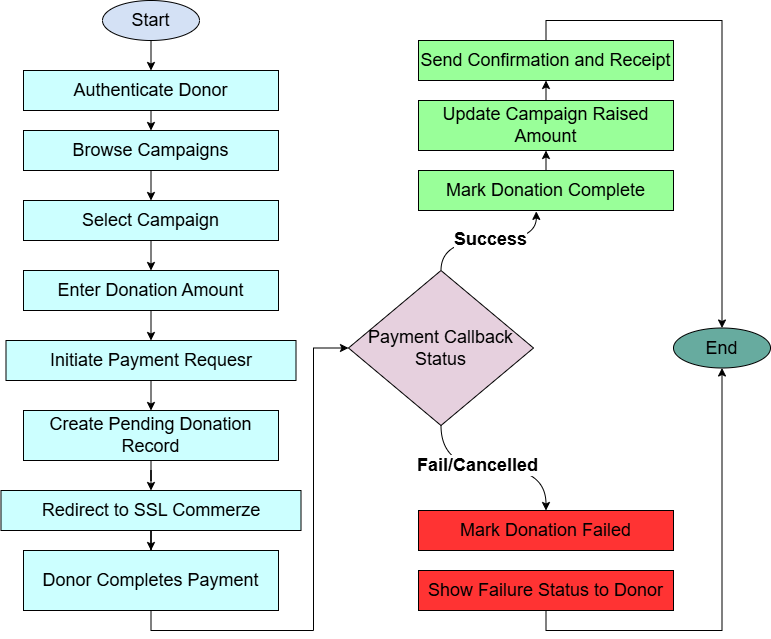
\includegraphics[%
            width=\dimexpr\linewidth-2\fboxsep-2\fboxrule\relax,%
            height=0.88\textheight,%
            keepaspectratio%
        ]{images/activity-diagram.png}}%
    }{%
        \fbox{\parbox[c][5cm][c]{\dimexpr\linewidth-2\fboxsep-2\fboxrule\relax}{%
            \centering\small Donation activity diagram image not available}}%
    }
    \caption{Activity Diagram for Donation Workflow.}
\end{figure}

\section{Campaign Lifecycle State Diagram}
Campaigns go through a series of states like Pending Approval, Active, Completed, and Canceled, but only some state transitions are permitted. The following diagram depicts these transitions. Logging of these state transitions and their authentication is mandatory to maintain accountability. For example, a campaign cannot be moved to an ‘Active’ state without any prior administration check. After a campaign attains a ‘Completed’ state, the process of fund settlement is initiated automatically.

\begin{figure}[H]
    \centering
    \screenshot{images/campaign_state_diagram.png}
    \caption{Campaign Lifecycle State Diagram.}
\end{figure}

\section{Authentication Flow}
Authentication relies on JWTs with role-aware authorization \cite{jones2015jwt}. Here is how the process works in practice.

\subsection{Registration, Login, and Token Issuance}
\begin{enumerate}
\item The password for a new user gets encrypted using BCrypt before storage.
    \item A token for email verification is created and emailed to the user’s email address.
    \item The server authenticates the user’s credentials at the time of login and sends back an access token as well as a refresh token.
    \item Upon expiration of the access token, the refresh token validates the token and generates a new access token without needing to authenticate the user again.
\end{enumerate}

\subsection{Authorization and Access Control}
After authentication, all requests to secured endpoints receive further scrutiny:
\begin{itemize}
    \item The JWT bearer middleware provided by ASP.NET Core verifies the integrity of the token's signature, issuer, audience, and expiration.
    \item Claims in the token are examined to ensure appropriate role constraints, meaning that only admin role tokens can access user management endpoints \cite{sandhu1996rbac}. 
    \item Any actions related to profile modification need the identity claim in the token to be equal to that of the targeted user.
\end{itemize}

\section{Payment Processing and Ledger Integration}
Monetary transactions occur via the SSLCommerz payment gateway, and the post-payment sync is managed by the backend using callback notifications \cite{hossain2019e}.
The gateway response is considered the ultimate authority for determining payment status, with ledger entries updated only when a valid callback notification occurs.
Each individual transaction gets entered in the immutable ledger entry form for auditing purposes.
A light retry mechanism is used to mitigate any temporary failure of callbacks.

\subsection{Sequence Diagram: Payment Callback Flow}
\begin{figure}[H]
    \centering
    \screenshot{images/payment_sequence_diagram.png}
    \caption{Sequence Diagram for Donation Payment Flow.}
\end{figure}

\subsection{How a Transaction Starts}
\begin{enumerate}
\item The donor hits the pay button on the frontend, triggering a server request.
    \item The class \texttt{PaymentController} creates a record for the donation with a status ``pending,'' along with an ID.
    \item Data about the payment such as amount, donor information, and callback URLs is sent to the SSLCommerz API.
    \item The browser of the user is then directed to the gateway URL provided by SSLCommerz.
\end{enumerate}

\subsection{Callback Handling and Idempotency}
After completing the process, or failing to pay, the payment is communicated back to the server by SSLCommerz:
\begin{itemize}
    \item The payload sent by the callback is mapped to the corresponding donation based on the donation ID or transaction reference.
    \item In case of a successful payment, the donation status changes to ``completed,'' changing from ``pending'' previously.
    \item The campaign total is updated, while anything above the target is allocated to the reserve fund row.
    \item To avoid any duplicate balance updates, idempotency check is performed for the callback.
\end{itemize}

\printchaptertitle{System Implementation}

\section{System Setup}
The operation of the system involves two main components: React-based frontend that runs statically, and backend written in ASP.NET Core providing an API as well as a connection to the database. The current section covers utilized technologies and implementation of all functionalities through screenshots.
Environment variables are used to separate environment-specific parameters like database connection strings and payment gateway keys for the development and production environments.
The backend application makes use of appsettings files and secrets manager to get access to environment variables without any hardcoding of credentials.
Entity Framework migrations help create the initial structure of the database, as well as reflect all changes in the source codebase.
The frontend assets are built using Vite and may be served along with the API itself or any web server.
Some scripts automate the process of starting both API and frontend in the local environment.
Specific endpoints are available for making health check calls verifying the connection to the database.

\subsection{Technologies Used}

\begin{itemize}
    \item \textbf{Frontend Technologies:}
\end{itemize}
\vspace{5pt}
\begin{table}[H]
    \centering
    \caption{Frontend Technologies.}
    \vspace{10pt}
    \begin{tabular}{|c|c|}
        \hline
        \textbf{SN} & \textbf{Technology} \\
        \hline
        1  & React \\
        2  & TypeScript \\
        3  & Redux Toolkit \\
        4  & Tailwind CSS \\
        5  & Axios (HTTP Client) \\
        6  & Vite (Build Tool) \\
        \hline
    \end{tabular}
\end{table}
\vspace{10pt}

\begin{itemize}
    \item \textbf{Backend Technologies:}
\end{itemize}
\vspace{5pt}
\begin{table}[H]
    \centering
    \caption{Backend Technologies.}
    \vspace{10pt}
    \begin{tabular}{|c|c|}
        \hline
        \textbf{SN} & \textbf{Technology} \\
        \hline
        1  & .NET Core 7/8 \\
        2  & C\# \\
        3  & Entity Framework Core \\
        4  & SQL Server \\
        5  & ASP.NET Core Identity \\
        6  & JWT Authentication \\
        \hline
    \end{tabular}
\end{table}
\vspace{10pt}

\section{System Implementation}

The screenshots that follow are in order exactly as they would be seen by a user: signing in, using the admin control panel, setting up campaigns, donating, and so forth. This will help in understanding how various aspects of the system interact in practice.

\subsection{User Authentication}
The login page is the starting point. What happens behind the scenes? Sessions using JWT technology provide authentication, emails confirm account validity, and refresh tokens ensure continuous user logins without the need for passwords each time.
An invalid login attempt is subject to rate limiting.
BCrypt is used to hash passwords that are never saved in plain text.
Logging out deactivates all refresh tokens.

\begin{figure}[H]
    \centering
    \screenshot{images/login.png}
    \caption{Login and Authentication Interface.}
\end{figure}

\subsection{Dashboard Overview}
Once logged into the system, a quick overview is available on the dashboard, which contains all the information that needs to be seen at once. This includes the total funds received, current active campaigns, pending reviews, and volunteer work.

\begin{figure}[H]
    \centering
    \screenshot{images/admin_dashboard.png}
    \caption{Admin Dashboard Overview.}
\end{figure}

\subsection{User and Role Management}
Admins can assign roles, enable or disable accounts, and manage user profiles from a dedicated panel.

\begin{figure}[H]
    \centering
    \screenshot{images/user_role.png}
    \caption{User and Role Management Panel.}
\end{figure}

\subsection{Campaign Management}
The creator of the campaign uses this interface to create new campaigns, set the amount needed, upload pictures, give updates on the progress and see how successful they have been in achieving their goals.
For easy categorisation in listings and search queries, a campaign needs a name, description, category, and target amount.
The start and end date of the campaign controls when it is exposed and prevents older campaigns from accepting donations.

Media files are checked for size and types to avoid slow loading times and improper file types.
We time-stamp campaigns for accountability and update them.
Administrators pause or archive campaigns if they break the rules or if they achieved their purpose.
Campaign status indicators to inform the user of the current status of a campaign.

\begin{figure}[H]
    \centering
    \screenshot{images/campaign_management.png}
    \caption{Campaign Creation and Management Interface.}
\end{figure}

\subsection{Donation Processing}
Donors go through a checkout flow that connects to SSLCommerz for payment. Once the transaction is confirmed, the system updates the donation status and campaign totals automatically.

\begin{figure}[H]
    \centering
    \screenshot{images/payment.png}
    \caption{Donation Checkout and Payment Initiation.}
\end{figure}

\subsection{Volunteer Management}
Volunteers have their own panel where they can submit activity reports, log hours, see their overall progress, and check how their contributions stack up.

\begin{figure}[H]
    \centering
    \screenshot{images/volunteer_panel.png}
    \caption{Volunteer Activity and Reporting Interface.}
\end{figure}

\subsection{Testimonial and Sentiment Analysis}
Donors who post testimonials are graded based on sentiment by the system. Any posts with negative sentiments are reviewed by the administration team before being displayed to the public. The sentiment analysis process is performed through machine learning models, which enable the system to determine whether the submitted content is of a positive, neutral, or negative nature. In doing so, the platform ensures that all donor testimonials displayed on its public forum do not contain any forms of inappropriate feedback. The moderation dashboard provides an interface where administrators have the opportunity to approve any comments that might offer constructive criticism but still be tagged as negative.

\begin{figure}[H]
    \centering
    \screenshot{images/testimonials.png}
    \caption{Testimonial Moderation and Sentiment Review.}
\end{figure}

\subsection{Analytics and Reporting}
The analytics dashboard pulls together donation trends, campaign performance, volunteer output, and donor activity into interactive charts and summary cards.

\begin{figure}[H]
    \centering
    \screenshot{images/analytics_dashboard.png}
    \caption{Analytics and Reporting Dashboard.}
\end{figure}

\subsection{Additional Feature Screenshots}
The remaining screenshots cover the other major modules built into the platform:

\begin{figure}[H]
    \centering
    \screenshot{images/campaign_updates.png}
    \caption{Campaign Updates and Announcement Interface.}
\end{figure}

\begin{figure}[H]
    \centering
    \screenshot{images/physical_donation.png}
    \caption{Physical Donation Verification and Tracking.}
\end{figure}

\begin{figure}[H]
    \centering
    \screenshot{images/expense_voucher.png}
    \caption{Expense Voucher Management and Approval Workflow.}
\end{figure}

\begin{figure}[H]
    \centering
    \screenshot{images/withdraw.png}
    \caption{Withdrawal Request and Approval Interface.}
\end{figure}

\begin{figure}[H]
    \centering
    \screenshot{images/reserve_fund.png}
    \caption{Reserve Fund Transparency.}
\end{figure}

\begin{figure}[H]
    \centering
    \screenshot{images/transaction_history.png}
    \caption{Payment Transaction History and Status Tracking.}
\end{figure}

\begin{figure}[H]
    \centering
    \screenshot{images/ML_insight.png}
    \caption{Machine Learning Insights and Prediction Outputs.}
\end{figure}

% \begin{figure}[H]
%     \centering
%     \screenshot{images/notification_center.png}
%     \caption{Notification and Communication Activity Interface.}
% \end{figure}

\subsection{Screenshot File Arrangement}
For consistency and maintainability, implementation screenshots should be stored under \texttt{Report/\allowbreak{}images} using the following filenames:

\begin{table}[H]
    \centering
    \caption{Implementation Screenshot Naming Scheme}
    \vspace{10pt}
    \begin{tabularx}{\linewidth}{|P{6.5cm}|L|}
        \hline
        \textbf{Filename} & \textbf{Purpose} \\
        \hline
        login\_page.png & Authentication/login screen. \\
        \hline
        admin\_dashboard.png & Main administrative overview and metrics. \\
        \hline
        user\_management.png & User, role, and access control management. \\
        \hline
        campaign\_management.png & Campaign create/update and progress monitoring. \\
        \hline
        donation\_checkout.png & Donation amount entry and payment initiation flow. \\
        \hline
        volunteer\_panel.png & Volunteer reporting and activity tracking. \\
        \hline
        testimonial\_moderation.png & Sentiment-based moderation and feedback review. \\
        \hline
        analytics\_dashboard.png & Reports and analytical visualizations. \\
        \hline
        campaign\_updates.png & Campaign announcement and progress update page. \\
        \hline
        physical\_donation.png & Physical donation collection and OTP verification workflow. \\
        \hline
        voucher\_management.png & Expense voucher submission and approval panels. \\
        \hline
        withdrawal\_management.png & Withdrawal request queue and administrative decisions. \\
        \hline
        reserve\_fund\_dashboard.png & Public reserve fund summary and transaction visibility. \\
        \hline
        payment\_transactions.png & Payment status log, callback result, and transaction history. \\
        \hline
        ml\_predictions.png & Forecasting, anomaly, and churn prediction outputs. \\
        \hline
        % \hline
        % notification\_center.png & Email/SMS/alert history and delivery status view. \\
        % \hline
    \end{tabularx}
\end{table}

\section{Key Features Implementation}

\subsection{Donation Tracking and Processing}
The donors and campaigners will receive real-time statistics on the amount of money collected for the goal. Every donation is stamped with the time, the amount of money donated and whether or not the transaction was successful. The module will be integrated with SSLCommerz for automatic generation of receipts and checking transactions.

\subsection{Campaign Updates and Communications}
Campaign creators post progress reports like stories about how donations are being used, achievements or even messages of gratitude. This keeps donors involved even after they’ve made their donations.

\subsection{Volunteer Reporting and Recognition}
The volunteers record their contributions through submission of reports detailing their hours of contribution, the nature of the contribution, campaigns they supported, and any outstanding achievement during the process. This information is used to rank the volunteers based on merits.

\subsection{Physical Donation Management}
In-kind contributions such as clothing, food, and materials are managed by the tracking module as follows:
\begin{itemize}
    \item OTP based authentication of donors using SMS.
    \item Documentation and evaluation of contributions.
    \item Linking to the donation ledger system.
    \item Creation of audit trails.
\end{itemize}

\subsection{Expense Voucher Management}
Vouchers are used for campaign-related expenses in the following way:
\begin{itemize}
    \item Structured vouchers, with documentation of all expenses.
    \item Approval hierarchies.
    \item Attachment of supporting documents.
    \item Status updates in real time.
\end{itemize}

\subsection{Control on Finance and Withdrawals}
No finance is withdrawn from the system unaccounted for:
\begin{itemize}
    \item Withdrawal request procedures.
    \item Authorization processes.
    \item Dashboard showing the status of public reserve funds.
    \item Notification mechanisms.
\end{itemize}

\subsection{Payment Integration}
SSLCommerz Payment Gateway offers support for credit card payments, mobile banking (bKash, Nagad), and digital wallets. Transactions are automatically confirmed by server callbacks; thus, nothing is required from the donor or administrator after the transaction.

\subsection{Machine Learning Features}
Every functionality in ML is hosted within the backend as an in-process \texttt{MLPredictionService} powered by ML.NET framework. It is registered as a singleton service; hence, once the model is trained, it stays in memory, and there is no need for training each time.

\subsubsection{1. Donation Demand Forecasting (SSA)}
Weekly donations are input into the SSA pipeline from ML.NET for forecasting along with their confidence intervals \cite{chen2022machine,hassani2007singular}. This allows the campaign managers to estimate the income they can expect during the upcoming weeks.

\subsubsection{2. Donor Attrition Prediction}
To classify potential donor attrition cases, the solution uses a binary classifier that includes variables such as the recency of the last gift, number of gifts, gift averages, and frequencies \cite{gupta2020donor}. It outputs a risk score along with an interpretable risk level (low, medium, high).

The probability estimate is interpreted as:
\begin{equation}
    P(Attrition) = \sigma\!\left(\sum_{i=1}^{n} w_i f_i\right)
\end{equation}
where $\sigma$ denotes the sigmoid mapping to a value in $[0,1]$.

\subsubsection{3. Donation Anomaly Detection}
The IID Spike Detection technique implemented in ML.NET identifies any anomalies in the finished donation data streams. Examples of what may be detected by this technique are:
\begin{itemize}
    \item Donations which are unusually large (small) compared to the campaign’s usual donations;
    \item Periods of unusual high activity inconsistent with the behavior of the campaign.
\end{itemize}
Any identified anomalies will appear in the admin dashboard.

\subsubsection{4. Sentiment Analysis}
The testimonial text gets classified into sentiments of positive, neutral, or negative by means of logistic regression using SDCA classifier algorithm. Any testimonial that gets classified into the negative class is automatically flagged for moderation purposes \cite{hutto2014vader}.

\subsubsection{5. Campaign and Volunteer Intelligence}
The software can also predict the likelihood that a particular campaign will achieve its objective and assign appropriate volunteers to assist in the process. The volunteering suggestions will be made using a composite score based on campaign traits and volunteer performance.

\subsection{Email and SMS Notifications}
Notification types include:
\begin{itemize}
    \item E-mail based confirmation of donation receipt.
    \item Campaign updates.
    \item Approvals/Rejections from administrative side.
    \item One-Time Password (OTP) delivery through SMS for donor authentication.
    \item Event-driven real-time notifications.
\end{itemize}

\subsection{Testimonial Moderation}
As mentioned in the ML section, testimonials with negative sentiment are flagged automatically. Admins can approve, edit, or reject them before they appear on the public-facing campaign pages.

\printchaptertitle{System Evaluation and Results}

\section{System Evaluation Overview}
To ensure that the system operates as it was supposed to, both automated and manual tests were carried out on the system. The test was aimed at verifying the functionality of the different parts of the system such as authentication, donation, volunteers management, testimonials moderation, and API analytics.

\section{Automated Test Coverage}
Both frontend and backend parts of the application have executable test suites. The table below summarizes what each layer validates.

\begin{table}[H]
    \centering
    \caption{Implemented Evaluation Layers}
    \vspace{10pt}
    \begin{tabularx}{\linewidth}{|P{4cm}|P{3.5cm}|L|}
        \hline
        \textbf{Evaluation Layer} & \textbf{Primary Tools} & \textbf{Validation Scope} \\
        \hline
        Frontend Unit/Component & Vitest, React Testing Library & UI behavior, reducers, and client service logic. \\
        \hline
        Frontend Contract & MSW & Contract-level checks for API wrapper behavior and payload handling. \\
        \hline
        Backend Unit/Integration & xUnit, Moq & Controller and service behavior under success and error conditions. \\
        \hline
        End-to-End & Playwright & End-user flows from login through dashboard and donation paths. \\
        \hline
    \end{tabularx}
\end{table}

\section{Functional Validation Scenarios}
The most critical business workflows were tested through a mix of API-level checks and manual end-to-end runs:

\begin{table}[H]
    \centering
    \caption{Critical Workflow Validation}
    \vspace{10pt}
    \begin{tabularx}{\linewidth}{|P{6.5cm}|l|L|}
        \hline
        \textbf{Workflow} & \textbf{Validation Type} & \textbf{Expected Outcome} \\
        \hline
        Registration and login & Automated + manual & Valid account creation, token issuance, and protected-route access. \\
        \hline
        Donation and payment callback & Manual integration & Pending donation updates to completed on successful callback. \\
        \hline
        Volunteer and reporting modules & API + UI checks & Report submission and status transitions operate correctly. \\
        \hline
        Testimonial moderation and analytics & API tests & Sentiment analysis and moderation states are persisted and retrievable. \\
        \hline
    \end{tabularx}
\end{table}

\section{ML Endpoint Validation}
For each ML module, there is an associated API call within the \texttt{MLController}. For the purposes of testing, we made calls to each of these end points using sample data:
\begin{itemize}
    \item \textbf{Forecasting:} Predictions of weekly donations along with confidence interval.
    \item \textbf{Sentiment:} Text classification and sentiment score.
    \item \textbf{Donor Churn:} Scored predictions for donor churn.
    \item \textbf{Campaign Success:} Estimated probability of success of campaigns.
    \item \textbf{Anomaly Detection:} Report of any anomalies in donation streams.
\end{itemize}

\section{Limitations and What Comes Next}
This build satisfies the core functional requirements; however, there are still areas for improvement prior to any actual production deployment. Some of the issues and the subsequent actions to be taken are outlined below:
\begin{itemize}
    \item \textbf{Performance testing:} Testing for performance and scalability was done, but load, soak, and concurrency testing were not performed.
    \item \textbf{Latency and throughput measurement:} Latency budget and throughput metrics have yet to be determined, so performance optimization targets will still remain speculative.
    \item \textbf{Validation dataset size:} The current model was tested using relatively small datasets that should be expanded to verify model generalization.
    \item \textbf{ML model drift detection:} No mechanism for periodic testing and retraining exists, which is crucial for reliable long-term use.
    \item \textbf{Penetration testing:} The basic security measures are implemented, but no penetration testing has been performed yet.
    \item \textbf{Operational readiness:} Basic observability is in place, but structured tracing, threshold-based alerting, and incident handling playbooks have not been developed.
    \item \textbf{Payment resiliency:} Callbacks are managed appropriately, but failure simulation for retries and gateway failure is still incomplete.
    \item \textbf{Data governance:} Retention policies and archival workflow requirements have not been defined formally.
\end{itemize}
Tackling these issues will transform the current validated prototype into a fully deployable platform with explicit performance and reliability SLAs.

\printchaptertitle{Conclusion and Future Work}

\section{Overview}
This chapter concludes the report with a brief overview of what was developed and its importance. First, it provides an overview of the capabilities provided by the tool, emphasizing its benefits in terms of transparency and efficiency. Then, it mentions the main limitations of the tool after validation, indicating the areas where further analysis of its performance, security, and machine learning capabilities is required. Finally, the chapter describes the improvements that could be made to make it more useful.

\section{Conclusion}

Considering the initial goals in terms of functionality and features to be implemented, it can be noted that the system has developed into quite a complex one. Indeed, it is able to provide users with all the features necessary for any charity campaign on a university campus, from gathering donations to managing finances and recruiting volunteers. Moreover, it has features that no other similar systems have.

A quick summary of what the system delivers:
\begin{itemize}
    \item \item \textbf{Donations Management:} Secure, instant transactions via SSLCommerz, receipts creation upon completion, and automatic updates for campaign totals.
    \item \textbf{Campaign Transparency:} Real-time tracking of progress and donation, sharing campaign information and a public reserve pool that makes donors know how their money will be spent.
    \item \textbf{Support for Volunteers:} Logging of activities and hours spent, and rewarding regular volunteers with a ranking system.
    \item \textbf{Insights From ML Algorithms:} Forecasting donations, anomalies detection, donor churn scoring, and sentiment analysis within the application backend.
    \item \textbf{Financial Management:} Vouchers should be approved before money transfer, formal withdrawal requests from the account, and full audit tracking.
    \item \textbf{Tracking of Physical Donations:} In-kind donations logging, valuation, and posting to the financial ledger.
    \item \textbf{Moderation of Testimonials:} Sentiment analysis algorithm detects sensitive posts and reports them to admins.
    \item \textbf{RBAC Implementation:} Proper role-based access control allows users from various roles to have limited permissions.
    \item \textbf{Multi-device Compatibility:} Mobile, tablet, and desktop interfaces conform to accessibility guidelines.
\end{itemize}

The tech stack of ASP.NET Core, React, SQL Server, and Redux Toolkit performed very well. The tech stack has grown mature enough for production use and can scale well. The security features were incorporated at an early stage of development. These include JWT authentication, BCrypt encryption of passwords, server validation, and cross-origin resource sharing restrictions. None of these features are cutting-edge technologies, but they cover all OWASP recommendations and help earn donor confidence.
At the very least, what I have learned through this exercise is that the manual way of doing things for campus fundraising can easily be done using software, which would make the process easier, cleaner, and more efficient.

\section{Future Work}

The current system is functional, but there is plenty of room to grow. Some directions worth pursuing:

\begin{itemize}
    \item \item \textbf{Multilingual Support:} Making the user interface and notifications in Bangla and other languages will enhance the accessibility of the platform. Furthermore, sentiment analysis should be multilingual.
    \item \textbf{Enhanced ML Models:} Although the models used are adequate, experimenting with other datasets and deep learning architectures like neural networks can increase accuracy.
    \item \textbf{Blockchain:} A blockchain system will increase transparency by recording all donations in an immutable ledger.
    \item \textbf{Recommendation Engine:} Donors will likely make more donations when recommended to specific campaigns in line with their previous activities on the site.
    \item \textbf{ERP Integration:} Universities and organizations have enterprise resource planning (ERP) software for accounting purposes. It may be useful to incorporate DMS with those systems and avoid duplicate data entry.
    \item \textbf{Mobile Application:} A native Android and iOS application will increase usability and allow for offline donation management for volunteers.
    \item \textbf{Customizable Queries:} Admins will be able to query the database themselves and export information in any desired format, thus avoiding manual work with Excel.
    \item \textbf{Social Impact Analysis:} The introduction of social return on investment will allow all stakeholders to evaluate the impact of campaigns on society in addition to the financial figures.
\end{itemize}

\subsection{Suggested Roadmap}
Rolling these out in phases keeps the work manageable:

\begin{table}[H]
    \centering
    \caption{Future Enhancement Roadmap}
    \vspace{10pt}
    \begin{tabularx}{\linewidth}{|P{3cm}|P{5.5cm}|L|}
        \hline
        \textbf{Phase} & \textbf{Primary Deliverables} & \textbf{Expected Outcome} \\
        \hline
        Phase 1 (0--3 months) & Security hardening, expanded test automation, and observability dashboards. & Improved reliability and reduced regression risk in production releases. \\
        \hline
        Phase 2 (3--6 months) & Mobile optimization, multilingual support, and reporting enhancements. & Higher accessibility and better stakeholder communication across user groups. \\
        \hline
        Phase 3 (6--12 months) & Advanced personalization and stronger ML models using larger historical datasets. & Better donor retention and improved forecasting quality. \\
        \hline
        Phase 4 (12+ months) & External ERP integrations and optional transparency-ledger extensions. & Stronger institutional interoperability and long-term governance maturity. \\
        \hline
    \end{tabularx}
\end{table}

Each phase builds on the previous one, so the system gets more capable over time without needing a risky ``big bang'' release.

\renewcommand{\bibname}{References}

\cleardoublepage
\thispagestyle{empty}

\vspace*{\fill}
\begin{center}
    \Huge \bfseries References
\end{center}
\vspace*{\fill}

\addcontentsline{toc}{chapter}{\textbf{References}}

% \nocite{*}  % Removed: only cited works should appear in the bibliography

\bibliographystyle{unsrt}
\bibliography{references}

\end{document}